% !Mode:: "TeX:UTF-8"
\chapter{相关技术}


\section{计算图}

目前的主流深度学习框架大多基于反向传播的方式来更新参数,计算图(Compute Graph)使得这一机制成为可能。计算图是一个有向无环图(DAG),深度学习框架把用户定义的算子保存为一个计算图,在反向传播时沿着计算图的边进行梯度的更新。同时目前主流的深度学习编译器也采用计算图作为中间表示,这种设计可以使得编译器的前端和后端进行分离,前端处理不同计算图之间的转换,把不同框架的计算图转换为统一表示的计算图,同时进行计算图层面的优化。后端把统一表示的计算图生成具体硬件可执行的代码。

下面的代码\ref{pytorch_model}具体定义一个模型来展示该模型生成的计算图。

\begin{lstlisting}[
    language={python},
    caption={Pytorch模型},
    label={pytorch_model},
]
import torch

class Model(torch.nn.Module):
    def __init__(self):
        super(Model, self).__init__()

        self.conv = torch.nn.Conv2d(3, 10, 3)
        self.fc = torch.nn.Linear(90, 10)

    def forward(self, x):
        # x shape [1, 3, 5, 5]
        x = self.conv(x)
        # x shape [1, 10, 3, 3]
        x = torch.flatten(x, 1)
        # x shape [1, 90]
        x = self.fc(x)
        # x shape [1, 10]

        return x
\end{lstlisting}

该模型仅由一个卷积和一个全连接层组成,输入向量的维度为(1, 3, 5, 5),输出向量的维度为(1, 10),可以通过下面的代码\ref{pytorch_scripted_model}来获得该模型的计算图。

\begin{lstlisting}[
    language={python},
    caption={Pytorch计算图},
    label={pytorch_scripted_model}
]
mod = Model()
scripted_model = torch.jit.trace(mod, torch.randn([1, 3, 5, 5]))
graph = scripted_model.graph.copy()

print(graph)
\end{lstlisting}

得到的计算图如下\ref{scripted_model_out}。

\begin{lstlisting}[
    language={},
    caption={计算图},
    label={scripted_model_out}
]
graph(%self.1 : __torch__.Model,
      %input.1 : Float(1, 3, 5, 5, strides=[75, 25, 5, 1], requires_grad=0, device=cpu)):
  %2 : __torch__.torch.nn.modules.linear.Linear = prim::GetAttr[name="fc"](%self.1)
  %3 : __torch__.torch.nn.modules.conv.Conv2d = prim::GetAttr[name="conv"](%self.1)
  %4 : Tensor = prim::CallMethod[name="forward"](%3, %input.1)
  %5 : int = prim::Constant[value=1]()
  %6 : int = prim::Constant[value=-1]()
  %input : Float(1, 90, strides=[90, 1], requires_grad=1, device=cpu) = aten::flatten(%4, %5, %6)
  %8 : Tensor = prim::CallMethod[name="forward"](%2, %input)
  return (%8)
\end{lstlisting}

该计算图的每一行是计算图中的一个节点,其中从左到右依次是节点变量,变量类型,以及该节点的操作(Operation)。


\section{RPC}


RPC(Remote Procedure Call),远程进程调用,是一个请求-回复的网络协议。在分布式的计算中,一台计算机中的进程往往需要调用另一台计算机中的进程,于是就诞生了RPC协议。RPC的流程如上图\ref{rpc}所示,客户端的进程向服务端发送一个包含参数的信息,并指定服务端执行一个特定的进程,服务端的进程执行完后把返回值发送消息给客户端。在服务端执行进程的过程中,客户端的进程通常是阻塞的,等到收到服务端返回的消息后在继续执行。同时通过RPC,客户端可以像调用本地进程一样调用远程的进程,而不需要额外的代码。

\begin{figure}[h!]
    \centering
    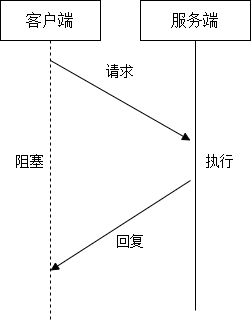
\includegraphics[width=180bp]{figure/rpc.png}
    \caption{RPC结构}
    \label{rpc}
\end{figure}

在本平台的实现过程中,为了把模型生成的可执行代码部署到具体硬件设备上,需要本地的进程和具体的硬件设备进行通信。一方面需要通过网络把编译好的模型发送到远程设备上,另一方面,本地进程需要通过RPC来通知具体的硬件设备来执行生成的可执行代码。下面的代码\ref{rpc_android}具体展示了如何通过RPC来调用安卓设备来执行生成的代码。

\begin{lstlisting}[
    language={Python},
    caption={RPC调用安卓},
    label={rpc_android}
]
# tracker\_host: RPC进程的IP地址,tracker\_port: RPC进程的端口,key: 是指定的关键字
tracker = rpc.connect_tracker(tracker_host, tracker_port)
remote = tracker.request(key)
# 上传生成的可执行代码到安卓设备,net.so是生成的动态链接库
remote.upload('net.so')
# 通知远程设备加载动态链接库并执行
rlib = remote.load_module('net.so')
\end{lstlisting}

在上面的代码中,首先使用RPC库,通过指定RPC服务端进程的IP地址和端口号来进行网络通信,获得远程设备的对象后,就可以通过调用该对象的一些函数来进行上传和执行生成代码等操作。


\section{TVM}

TVM是一个端到端的神经网络模型的编译器工具链,支持目前主流的前端的深度学习框架,如Pytorch,Tensorflow,Caffe等,同时支持部署到广泛的后端硬件设备,如CPU,服务器端GPU,移动端GPU,FPGA等。在编译过程中TVM同时对模型进行优化,分别进行高层次的计算图优化和低层次的硬件相关的算子优化来保证部署到硬件设备上的模型的效率。

\begin{figure}[h!]
    \centering
    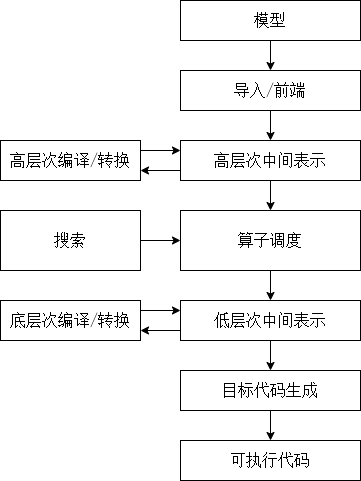
\includegraphics[width=180bp]{figure/tvm.png}
    \caption{TVM编译流程}
    \label{tvm_compile}
\end{figure}

TVM的整体编译流程如上图\ref{tvm_compile}所示,首先TVM的前端导入深度学习框架的模型,在这一过程中,TVM通过预先设定的算子(Operation)的映射,把不同深度学习框架计算图的算子转换为统一的算子,得到IR(Intermediate Representation),中间表示。同时对中间表示进行一些优化,如常数合并,死代码消除,向量维度转化等。这些优化大多和具体的硬件架构无关。以模型\ref{pytorch_model}为例,其计算图为\ref{scripted_model_out},在经过TVM前端的编译后得到的计算图如下\ref{relay_function}。

\begin{lstlisting}[
    language={},
    caption={TVM计算图},
    label={relay_function}
]
fn (%input0: Tensor[(1, 3, 5, 5), float32], %conv.weight: Tensor[(10, 3, 3, 3), float32], %conv.bias: Tensor[(10), float32], %fc.weight: Tensor[(10, 90), float32], %fc.bias: Tensor[(10), float32]) {
  %0 = nn.conv2d(%input0, %conv.weight, padding=[0, 0, 0, 0], channels=10, kernel_size=[3, 3]);
  %1 = nn.bias_add(%0, %conv.bias);
  %2 = reshape(%1, newshape=[0, -1, 1, 1]);
  %3 = squeeze(%2, axis=[2, 3]);
  %4 = transpose(%fc.weight, axes=[1, 0]);
  %5 = transpose(%4, axes=[1, 0]);
  %6 = nn.dense(%3, %5, units=10);
  add(%6, %fc.bias)
}
\end{lstlisting}

在得到高层次的中间表示后,TVM会把高层次的中间表示转换为底层次的中间表示,并对低层次的中间表示进行一些优化,其中的优化分为两种,一种是确定的基于规则的优化,另一种是采用机器学习的方法搜索出更优的优化方案。这些优化大多是和具体的硬件架构相关的。其中,确定的优化包括多维数组的寻址展开为一维的数组寻址,把算子展开为具体硬件相关的元语等。但是,不同的硬件在支持的元语和内存架构等方面都有所不同,所以很难通过确定的优化方案对每种硬件都有很好的支持,为了支持更多的硬件和更好的效率,TVM采用了基于搜索和学习的优化方案。TVM首先定义了一些调度的元语,例如循环转化(Loop Transformations),代码内连(Inline),向量化(Vectorization)等。TVM在一定的搜索空间内搜索出效率更好的调度方案。

在对低层次中间表示进行优化后,TVM针对具体的硬件进行代码的生成。TVM通过调用一些其他的编译器,如LLVM来生成一些CPU可执行的代码,同时也可以生成一些Cuda和OpenCL的源代码。最后TVM提供了一个轻量化的运行库(Runitme)来调用和执行生成的代码。


\section{VTA}


VTA(Versatile Tensor Accelerator)是一个统一的,可定制的深度学习加速器,并对TVM编译栈有很好的支持,VTA和TVM一起可以提供一个端到端的硬件到软件的深度学习栈。

VTA具有以下特点:
\begin{itemize}
    \item {统一,模块化。}
    \item {方便部署到FPGA设备上。}
    \item {提供了模拟器可以快速搭建原型。}
    \item {集成了TVM编译栈。}
\end{itemize}

\begin{figure}[h!]
    \centering
    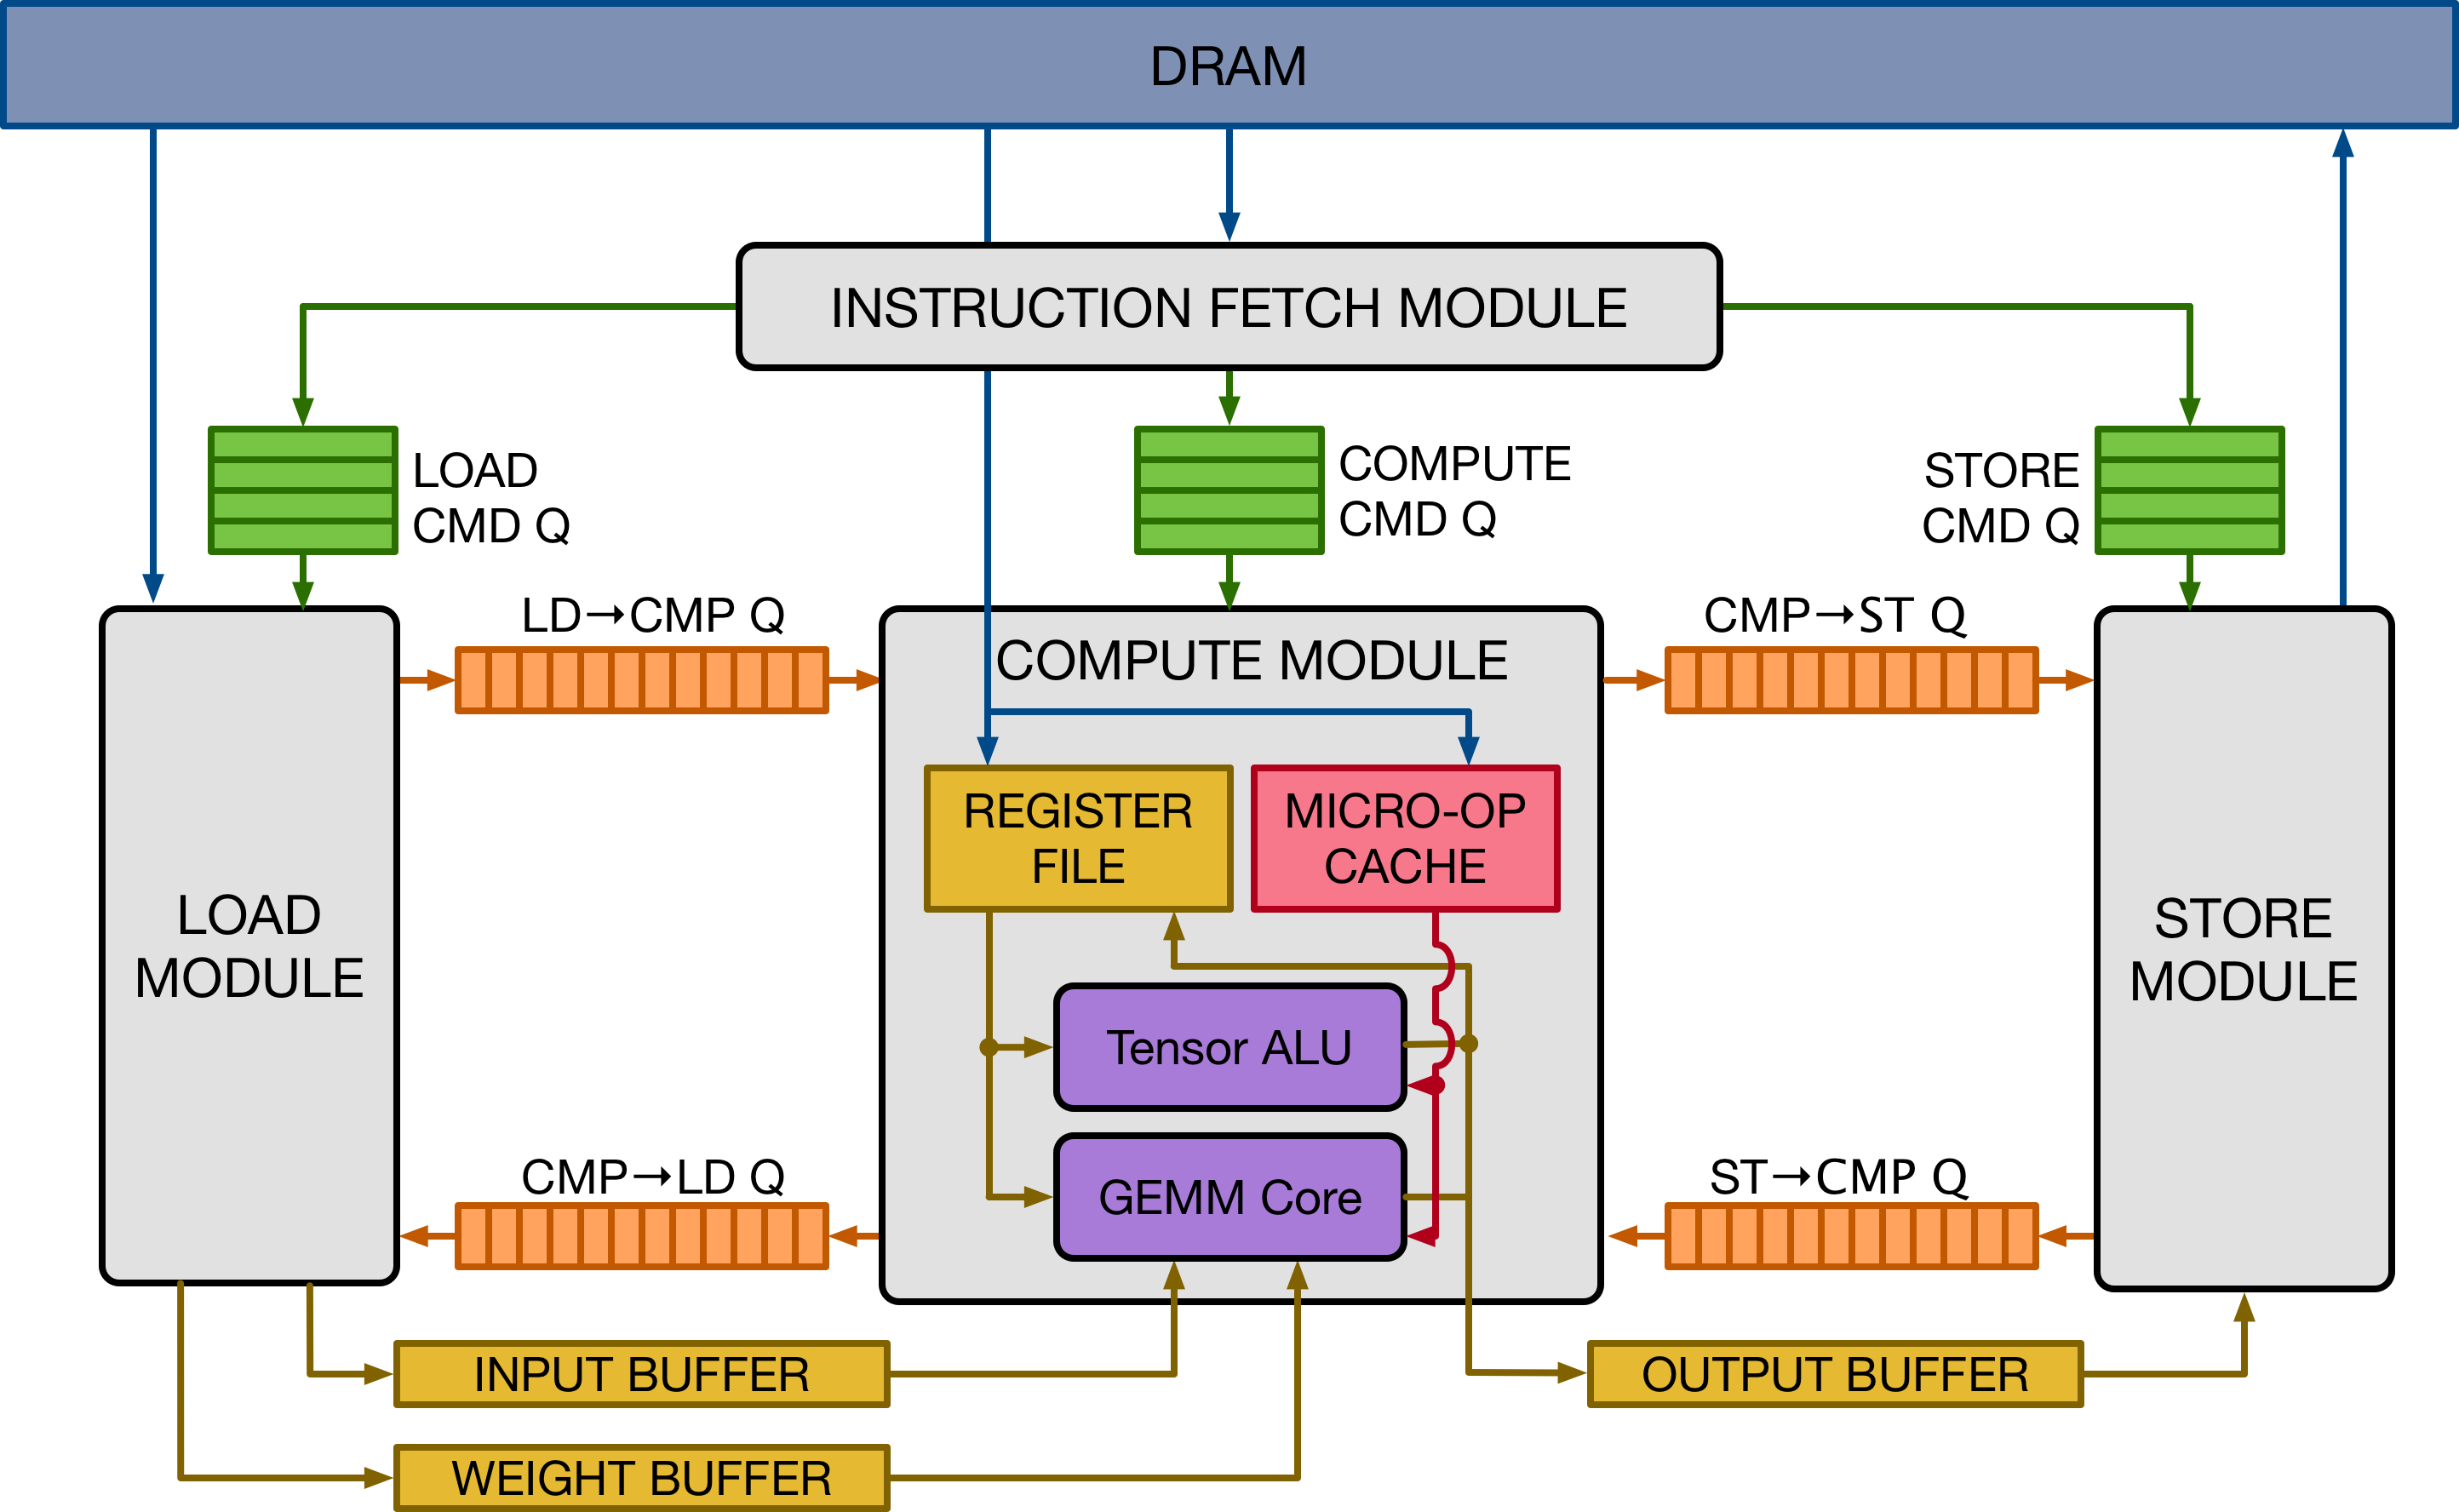
\includegraphics[width=270bp]{figure/vta_overview.png}
    \caption{VTA结构}
    \label{vta}
\end{figure}

如上图\ref{vta}所示,VTA整体分为四个模块,获取模块(Fetch Module),加载模块(Load Module),计算模块(Compute Module),储存模块(Store Module)。这些模块通过一些队列来进行通信。其中,获取模块负责从内存中获得指令序列,并对指令进行解码,把解码后的指令分别储存进其他三个模块队列(LOAD CMD Q,COMPUTE CMD Q,STORE CMD Q)中。加载模块负责从内存中读取输入和权重向量并储存到VTA的INPUT BUFFER(输入缓存)和WEIGHT BUFFER(权重缓存)中。计算模块负责通过它的GEMM Core(General Matrix Multiply)核心来进行一些矩阵的运算和通过其Tensor ALU来进行一些向量的计算,同时还负责从内存中读取一些数据储存到REGISTER FILE(向量寄存器)以及负责从内存中读取一些Micro-Op(微指令)储存到MICRO-OP CACHE(微指令缓存)中。储存模块负责把计算的结果储存回内存中。

VTA的指令集,ISA(Instruction Set Architecture),分为四类,LOAD,GEMM,ALU,STORE。LOAD指令负责从内存中读取一个2维的向量并把向量储存在INPUT BUFFER,WEIGHT BUFFER或REGISTER FILE中。GEMM指令可以执行一些Micro-Op,对输入矩阵和权重矩阵进行运算,并把结果储存在REGISTER FILE中。ALU指令执行一些矩阵与矩阵之间的一些操作。STORE指令负责把输出的向量储存回内存当中。